\chapter{Probleemanalyse}

\section{Probleemomschrijving}
Het project heet Satellite. Satellite is een nieuw project dat ontwikkeld wordt door Sensor Maritime als een data gedreven optimalisatie voor scheepvaart. Het geeft een kapitein de mogelijkheid om aan de hand van data kosten te besparen. Dit wordt gedaan door gegevens te verzamelen. Met deze data kan een kapitein efficiënter werken door veiliger, slimmer en duurzamer te opereren. Elke kapitein zal andere data willen voor zijn binnenvaartschip. Dit betekent dat het veranderen van sensoren simpel en snel moet zijn. Satellite (zie \ref{fig:shw} is zo ontwikkeld dat je plug en play verschillende sensoren kan toevoegen. Dit wordt gedaan door verschillende IO porten en connectors toe te voegen aan de hardware. De Satellite hardware is al ontwikkeld, maar mist alleen nog de software om als product het te gebruiken. Aan de afstudeerder is er gevraagd om voor de hardware, software te schrijven waarbij de nieuwe hardware gelijk getest kan worden. Hiervoor zal een testplan gemaakt moeten worden en een test applicatie ontwikkeld worden.
\begin{figure}[h!]
	\begin{centering}
		\caption{Satellite hardware}
	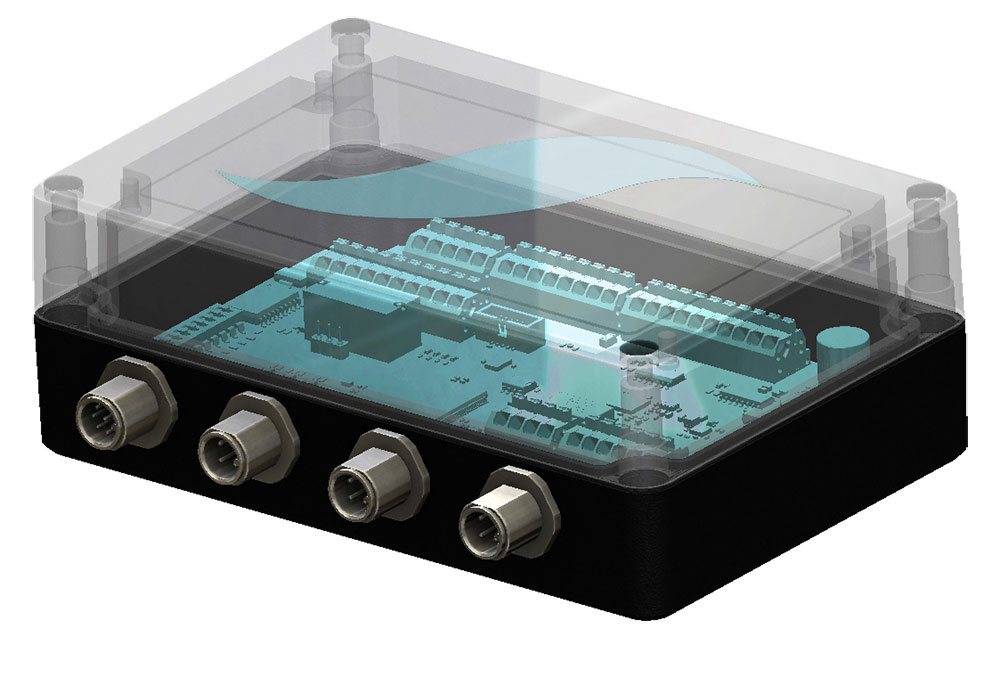
\includegraphics[width=0.35\linewidth]{statements/satellite.jpg}

	\label{fig:shw}
	\end{centering}
\end{figure}
\section{Betrokken partijen}
Tijdens de afstudeerstage zijn er twee partijen betrokken, Sensor Maritime in Vught en de student die de afstudeerstage volgt. Mark-Ivo van Ooijen van Sensor Maritime is de begeleider en projectleider. De tweede partij is de afstudeerder zelf, Patrick de Jong. Vanuit school zijn er ook 2 examinatoren, maar deze zijn niet betrokken bij het project zelf. De examinatoren zijn Andries van Dongen, hij is de een docentbegeleider die de afstudeerstage zal begeleiden. Pieter Kop Jansen zal er alleen zijn bij de uiteindelijke verdediging.

\section{Onderzoeksvraag}
De onderzoeksvraag tijdens de afstudeerstage zal zijn: \textbf{Hoe kan een modulair softwaresysteem worden ontwikkeld voor de Satellite hardware zo dat verschillende sensoren ondersteunt worden en data verstuurd kan worden naar een extern opslagpunt?}

\section{Deelvragen}
Voor het Satellite project zijn de volgende deelvragen gedefinieerd:
\begin{enumerate}
	\item Hoe kan er een robuuste  communicatie gecreëerd worden tussen het hoofdsysteem en Satellite?
	\item Op welke manier moet de software ontworpen worden zodat het makkelijk uitbreidbaar is voor nieuwe sensoren?
	\item Welke stappen zijn er nog om alle IO porten te testen van de Satellite?
\end{enumerate}

\section{Doelstellingen}
De doelstelling van het project geven duidelijkheid in wat er precies bereikt moet worden in betrekking met de onderzoeksvraag en deelvraag. Hieronder is een lijst dat aangeeft welke doelstellingen bereikt moeten worden.
\begin{enumerate}
	\item De Satellite IO porten zijn volledig getest, en kunnen communiceren met sensoren.
	\item De Satellite heeft een robuuste communicatie over CAN en UDP. 
	\item Generiek en modulair opgebouwd software, waardoor het in de toekomst makkelijk uitgebreid kan worden.
\end{enumerate}

\section{Eisen}
De volgende tabel \ref{tab:eisen} geeft een overzicht van de eisen voor het project Satellite.
\begin{table}[h!]
	\caption{MoSCoW Analyse}

	\resizebox{\textwidth}{!}{
		\begin{tabular}{|l | l |}
		\hline
		\multirow{5}{*}{\textbf{Must have}} 	& Alle IO porten van de Satellite moeten getest worden                                   	\\ \cline{2-2}
												& Implementatie van de hoekmeting en versnellingsassen                                   	\\ \cline{2-2}
												& Spectrum analyse maken van de versnellingassen                                         	\\ \cline{2-2}
												& Errors moeten goed afgevangen worden, de applicatie mag niet crashen of blijven hangen 	\\ \cline{2-2}
												& CAN implementatie, en correct protocol afhandeling                                     	\\ \hline
		\multirow{2}{*}{\textbf{Should have}} 	& Implementatie voor IO-Link sensoren                                                    	\\ \cline{2-2}
												& Hoogte sensoren en antenne sensor inlezen                                              	\\ \hline
		\multirow{2}{*}{\textbf{Could have}} 	& Standaard datastructuur voor paketten die worden opgestuurd 						   		\\ \cline{2-2}
												& Debug berichten worden opgestuurd via UDP/CAN                                          	\\ \cline{2-2}
		\multirow{3}{*}{\textbf{Won't have}}	& Ondersteuning van niet gekozen sensoren van Sensor Maritime  						   		\\ \hline
												& Ondersteuning voor andere communicatiemiddelen dan UDP, CAN								\\ \cline{2-2}
												& Ondersteuning voor andere embedded systemen                                        	   	\\ \hline  
	\end{tabular}%
	}
	\label{tab:eisen}
\end{table}

